\subsection{Diagramy sekwencji}
\begin{adjustwidth}{2em}{0pt}

W tym podrozdziale przedstawiono wybrane diagramy sekwencji. Diagram sekwencji obrazuje interakcje pomiędzy częściami systemu w postaci sekwencji komunikatów np. wywołań funkcji wymienianych między nimi. 

\begin{figure}[H]
    \centering
    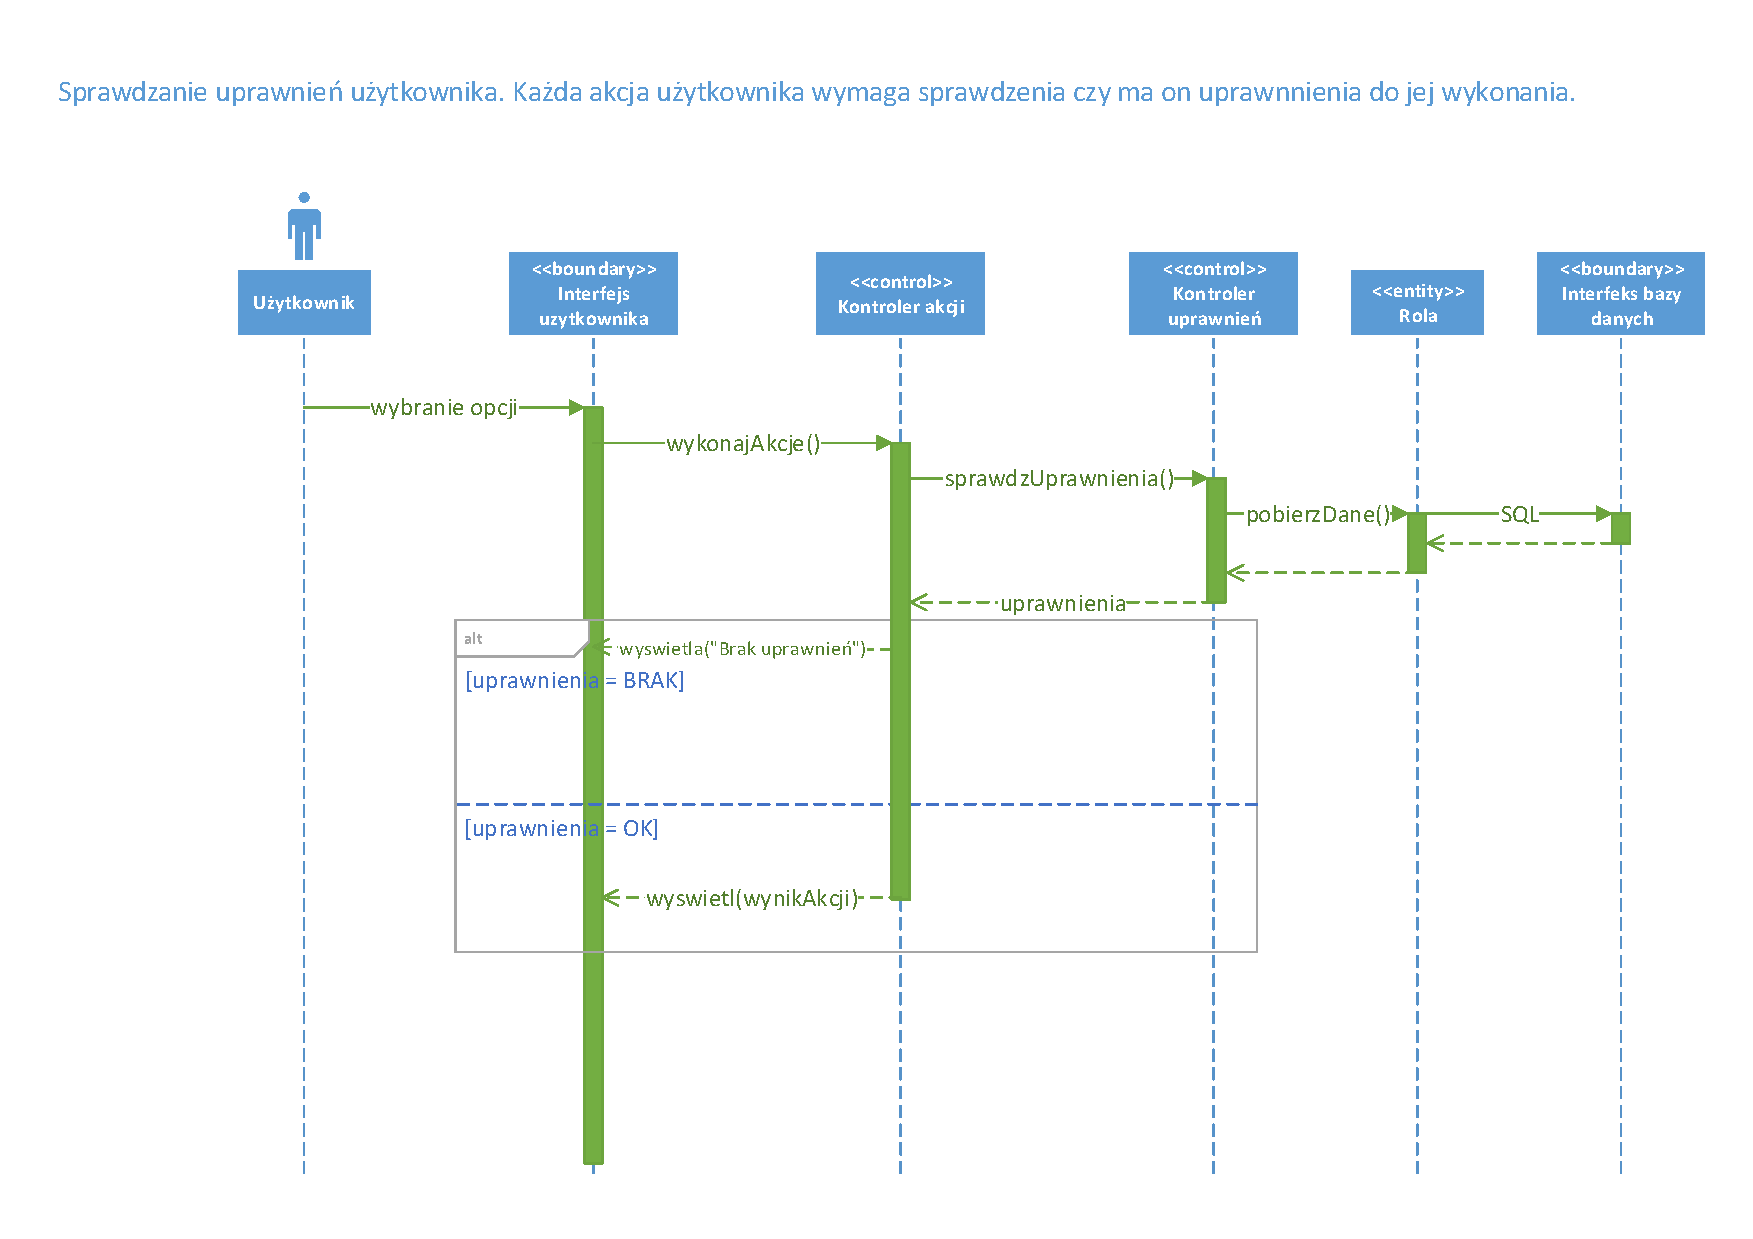
\includegraphics[scale=0.8, , angle=90 ]{diagramy/sekwencji_i_komponentow/seq_sprawdzanieUprawnien.pdf}
    \caption{Diagram sekwencji: Sprawdzanie uprawnień}
    \label{fig:seq_sprawdzanieUprawnien.pdf}
\end{figure} 

\begin{figure}[H]
    \centering
    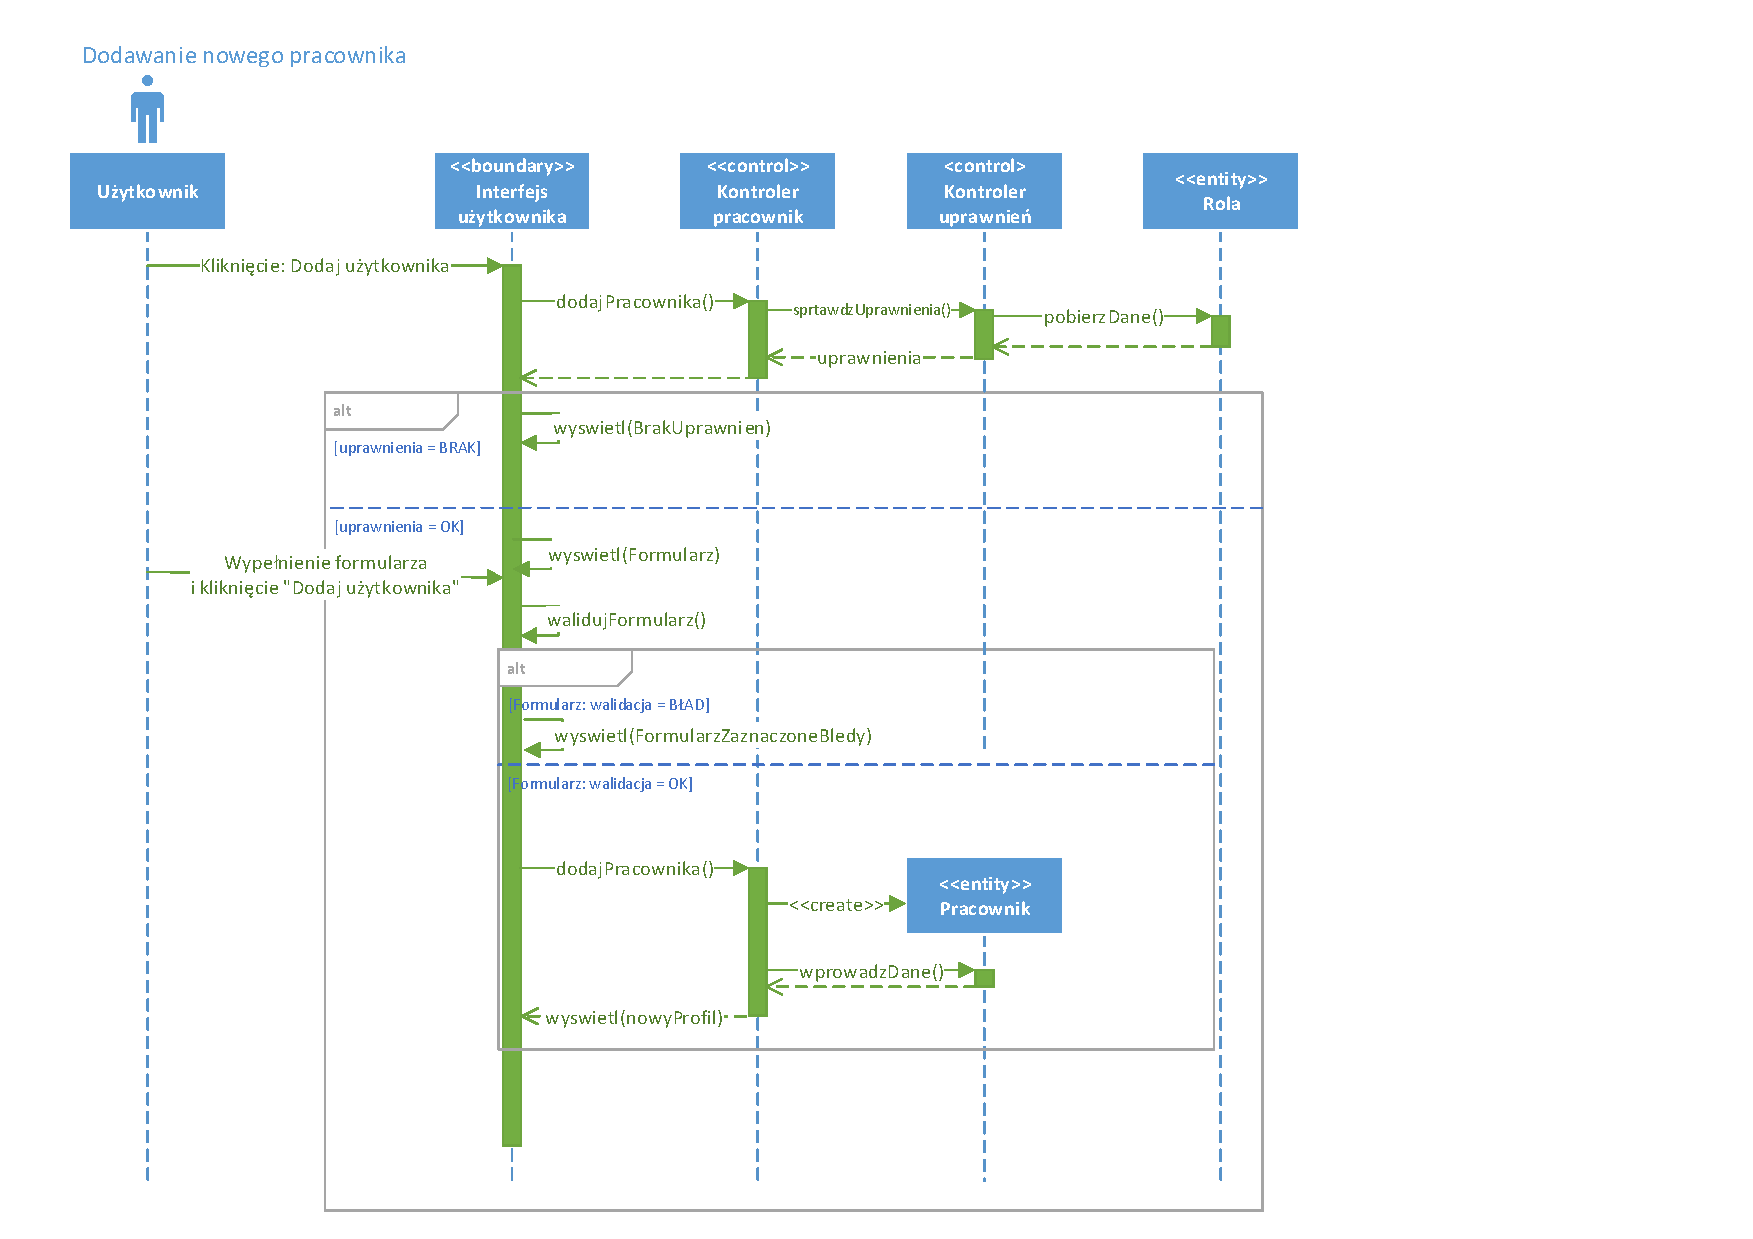
\includegraphics[scale=0.8, , angle=90]{diagramy/sekwencji_i_komponentow/seq_nowyPracownik.pdf}
    \caption{Diagram sekwencji: Dodawanie nowego pracownika}
    \label{fig:seq_nowyPracownik.pdf}
\end{figure} 

\begin{figure}[H]
\end{figure} 

\end{adjustwidth}
